\documentclass[12pt,letterpaper]{exam}
\usepackage[lmargin=1in,rmargin=1in,tmargin=1in,bmargin=1in]{geometry}
\usepackage{../style/exams}

% -------------------
% Course & Exam Information
% -------------------
\newcommand{\course}{MAT 104: Exam 2}
\newcommand{\term}{Spring -- 2023}
\newcommand{\examdate}{04/13/2023}
\newcommand{\timelimit}{85 Minutes}

\setbool{hideans}{false} % Student: True; Instructor: False

% -------------------
% Content
% -------------------
\begin{document}

\examtitle
\instructions{Write your name on the appropriate line on the exam cover sheet. This exam contains \numpages\ pages (including this cover page) and \numquestions\ questions. Check that you have every page of the exam. Answer the questions in the spaces provided on the question sheets. Be sure to answer every part of each question and show all your work.} 
\scores
%\bottomline
\newpage

% ---------
% Questions
% ---------
\begin{questions}

% Question 1
\newpage
\question[15] Complete the table of exact values for the trigonometric figures given below.
	{\def\arraystretch{3}
	\setlength{\tabcolsep}{2.5em}
	\begin{table}[!ht]
	\centering
	\begin{tabular}{|c||c|c|c|c|c|} \hline
	$\theta$ & $0$ & $\dfrac{\pi}{6}$ & $\dfrac{\pi}{4}$ & $\dfrac{\pi}{3}$ & $\dfrac{\pi}{2}$ \\ \hline \hline
	$\sin \theta$ & $0$ & $\dfrac{1}{2}$ & $\dfrac{1}{\sqrt{2}}$ & $\dfrac{\sqrt{3}}{2}$ & $1$ \\ \hline
	$\cos \theta$ & $1$ & $\dfrac{\sqrt{3}}{2}$ & $\dfrac{1}{\sqrt{2}}$ & $\dfrac{1}{2}$ & $0$ \\ \hline
	$\tan \theta$ & $0$ & $\dfrac{1}{\sqrt{3}}$ & $1$ & $\sqrt{3}$ & Undef. \\ \hline
	\end{tabular}
	\end{table}
	}



% Question 2
\newpage
\question[15] Compute the exact values for the trigonometric functions given below.
	\begin{enumerate}[(a)]
	\item $\cos \!\left( \dfrac{5\pi}{6} \right)$
	\item $\tan \!\left( \dfrac{4\pi}{3} \right)$
	\item $\sin \!\left( -\dfrac{7\pi}{4} \right)$
	\item $\tan \!\left( \dfrac{3\pi}{2} \right)$
	\item $\sec \!\left( \dfrac{\pi}{4} \right)$
	\item $\cot \left( \pi \right)$
	\item $\csc \!\left( \dfrac{2\pi}{3} \right)$
	\end{enumerate} \pspace

{\itshape \sol
\begin{enumerate}[(a)]
\item 
	\[
	\cos \!\left( \dfrac{5\pi}{6} \right)= -\cos \!\left( \dfrac{\pi}{6} \right)= -\dfrac{\sqrt{3}}{2}
	\]

\item 
	\[
	\tan \!\left( \dfrac{4\pi}{3} \right)= \tan \!\left( \dfrac{\pi}{3} \right)= \sqrt{3}
	\]

\item 
	\[
	\sin \!\left( -\dfrac{7\pi}{4} \right)= -\sin \!\left( \dfrac{7\pi}{4} \right)= - \left( - \sin \!\left( \dfrac{\pi}{4} \right) \right)= \dfrac{1}{\sqrt{2}}
	\]

\item 
	\[
	\tan \!\left( \dfrac{3\pi}{2} \right)= \text{undefined}
	\]

\item 
	\[
	\sec \!\left( \dfrac{\pi}{4} \right)= \dfrac{1}{\cos \!\left( \dfrac{\pi}{4} \right)}= \dfrac{1}{\dfrac{1}{\sqrt{2}}}= \sqrt{2}
	\]

\item 
	\[
	\cot \left( \pi \right)= \dfrac{1}{\tan \!\left( \pi \right)}= \dfrac{1}{0}= \text{undefined}
	\]

\item 
	\[
	\csc \!\left( \dfrac{2\pi}{3} \right)= \dfrac{1}{\sin \!\left( \dfrac{2\pi}{3} \right)}= \dfrac{1}{\sin \!\left( \dfrac{\pi}{3} \right)}= \dfrac{1}{\dfrac{\sqrt{3}}{2}}= \dfrac{2}{\sqrt{3}}
	\]
\end{enumerate}
}



% Question 3
\newpage
\question[10] Compute the exact values (in radians) for the inverse trigonometric functions given below.
	\begin{enumerate}[(a)]
	\item $\sin^{-1} \!\!\left( -\dfrac{1}{2} \right)$
	\item $\arccos \!\left( \dfrac{1}{2} \right)$
	\item $\tan^{-1} \!\left( -\sqrt{3} \right)$
	\item $\arcsin \!\left( \sin \left( \dfrac{7\pi}{6} \right) \right)$
	\item $\arctan(\infty)$
	\end{enumerate} \pspace

{\itshape \sol 
\begin{enumerate}[(a)]
\item 
	\[
	\sin^{-1} \!\!\left( -\dfrac{1}{2} \right)= -\dfrac{\pi}{6}
	\] \pspace

\item 
	\[
	\arccos \!\left( \dfrac{1}{2} \right)= \dfrac{\pi}{3}
	\] \pspace

\item 
	\[
	\tan^{-1} \!\left( -\sqrt{3} \right)= -\dfrac{\pi}{3}
	\] \pspace

\item 
	\[
	\arcsin \!\left( \sin \left( \dfrac{7\pi}{6} \right) \right)= \arcsin \!\left( -\sin \left( \dfrac{\pi}{6} \right) \right)= \arcsin \left( -\dfrac{1}{2} \right)= -\dfrac{\pi}{6}
	\] \pspace

\item 
	\[
	\arctan(\infty)= \dfrac{\pi}{2}
	\] 
\end{enumerate}
}
	


% Question 4
\newpage
\question[10] Given the right triangle below, compute the exact values of the indicated trigonometric functions. \pspace
\begin{minipage}{0.3\textwidth}
        \begin{enumerate}[(a)]
        \item $\sin \theta$
        \item $\cos \phi$
        \item $\tan \theta$
        \item $\sec \theta$
        \item $\csc \phi$
        \end{enumerate}
\end{minipage} \begin{minipage}{0.27\textwidth}        
	\[
	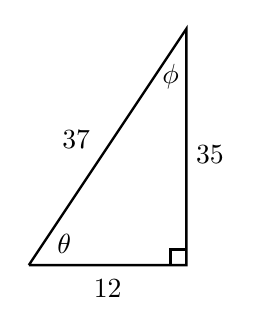
\begin{tikzpicture}
	\draw[line width=0.03cm] (0,0) -- (2,0) -- (2,3) -- (0,0);
	\draw[line width=0.03cm] (1.8,0) -- (1.8,0.2) -- (2,0.2);
	\node at (0.45,0.27) {$\theta$};
	\node at (1.8,2.4) {$\phi$};
	\node at (1,-0.3) {$12$};
	\node at (2.3,1.4) {$35$};
	\node at (0.6,1.6) {$37$};
	\end{tikzpicture}
	\]
\end{minipage} \pspace

{\itshape \sol 
\begin{enumerate}[(a)]
\item 
	\[
	\sin \theta= \dfrac{\text{opposite}}{\text{hypotenuse}}= \dfrac{35}{37}
	\] \pspace

\item 
	\[
	\cos \phi= \dfrac{\text{adjacent}}{\text{hypotenuse}}= \dfrac{35}{37}
	\] \pspace

\item 
	\[
	\tan \theta= \dfrac{\text{opposite}}{\text{adjacent}}= \dfrac{35}{12}
	\] \pspace

\item 
	\[
	\sec \theta= \dfrac{1}{\cos \theta}= \dfrac{1}{\dfrac{\text{adjacent}}{\text{hypotenuse}}}= \dfrac{\text{hypotenuse}}{\text{adjacent}}= \dfrac{37}{12}
	\] \pspace

\item 
	\[
	\csc \phi= \dfrac{1}{\sin \phi}= \dfrac{1}{\dfrac{\text{opposite}}{\text{hypotenuse}}}= \dfrac{\text{hypotenuse}}{\text{opposite}}= \dfrac{37}{12}
	\] 
\end{enumerate}
}



% Question 5
\newpage
\question[10] Showing all your work, compute the exact value of the expressions given below.
	\begin{enumerate}[(a)]
	\item $\sin(2\theta)$, if $\tan(\theta)= \dfrac{4}{3}$ and $0 < \theta < \dfrac{\pi}{2}$
	\item $\tan \!\left( \cos^{-1} \left( -\dfrac{3}{4} \right) \right)$
	\end{enumerate} 

{\itshape \sol 
% (a)
\begin{enumerate}[(a)]
\item 
\end{enumerate}
\begin{minipage}[c]{0.45\textwidth}
Because $0 < \theta < \frac{\pi}{2}$ is acute and using the fact that $\tan(\theta)= \text{opposite}/\text{adjacent}$, because $\tan(\theta)= \dfrac{4}{3}$, we can draw the following triangle on the left below:
	\[
	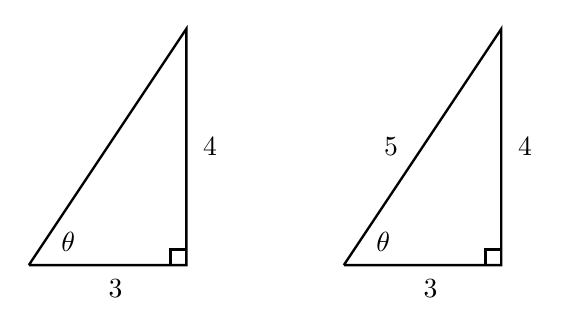
\begin{tikzpicture}
	\draw[line width=0.03cm] (0,0) -- (2,0) -- (2,3) -- (0,0);
	\draw[line width=0.03cm] (1.8,0) -- (1.8,0.2) -- (2,0.2);
	\node at (0.5,0.3) {$\theta$};
	\node at (2.3,1.5) {$4$};
	\node at (1.1,-0.3) {$3$};
	
	\tikzset{shift={(4,0)}}
	
	\draw[line width=0.03cm] (0,0) -- (2,0) -- (2,3) -- (0,0);
	\draw[line width=0.03cm] (1.8,0) -- (1.8,0.2) -- (2,0.2);
	\node at (0.5,0.3) {$\theta$};
	\node at (2.3,1.5) {$4$};
	\node at (1.1,-0.3) {$3$};
	\node at (0.6,1.5) {$5$};
	\end{tikzpicture}
	\]
Because the triangle is a right triangle, using the Pythagorean Theorem, we know that $a^2 + b^2= c^2$.
\end{minipage} \hspace{1cm} \begin{minipage}[c]{0.45\textwidth}
But then\dots
	\[
	\begin{gathered}
	a^2 + b^2= c^2 \\
	3^2 + 4^2= c^2 \\
	9 + 16= c^2 \\
	25= c^2 \\
	c= \sqrt{25} \\
	c= 5
	\end{gathered}
	\]
This gives the triangle on the right above. Finally, using the fact that $\sin \theta= \text{opposite}/\text{hypotenuse}$, $\cos \theta= \text{adjacent}/\text{hypotenuse}$, and $\sin(2\theta)= 2 \sin \theta \cos \theta$, we have\dots
	\[
	\sin(2\theta)= 2 \sin \theta \cos \theta= 2 \cdot \dfrac{4}{5} \cdot \dfrac{3}{5}= \dfrac{24}{25}
	\]
\end{minipage} 

% (b)
\begin{enumerate}[(b)]
\item 
\end{enumerate}
\begin{minipage}[c]{0.45\textwidth}
Suppose that $\theta= \cos^{-1}(-3/4)$. Applying cosine to both sides we have $\cos \theta= \cos \left( \cos^{-1}(-3/4) \right)= -\frac{3}{4}$. Replacing $\theta$ with its reference angle, using the fact that $0 \leq \cos^{-1}(x) \leq \pi$, $\cos \theta < 0$, and the fact that $\cos \theta= \text{adjacent}/\text{hypotenuse}$, because $\cos \theta= -\frac{3}{4}$, we can draw the triangle below.
	\[
	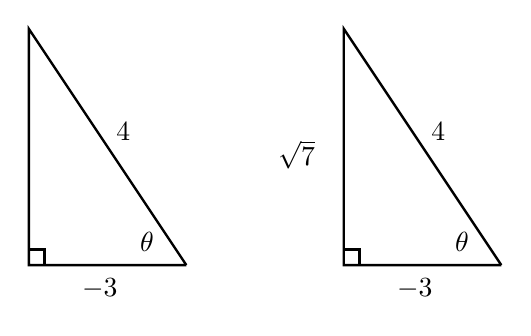
\begin{tikzpicture}
	\draw[line width=0.03cm] (0,0) -- (-2,0) -- (-2,3) -- (0,0);
	\draw[line width=0.03cm] (-1.8,0) -- (-1.8,0.2) -- (-2,0.2);
	\node at (-1.1,-0.3) {$-3$};
	\node at (-0.8,1.7) {$4$};
	\node at (-0.5,0.3) {$\theta$};

	\tikzset{shift={(4,0)}}

	\draw[line width=0.03cm] (0,0) -- (-2,0) -- (-2,3) -- (0,0);
	\draw[line width=0.03cm] (-1.8,0) -- (-1.8,0.2) -- (-2,0.2);
	\node at (-1.1,-0.3) {$-3$};
	\node at (-0.8,1.7) {$4$};
	\node at (-2.6,1.4) {$\sqrt{7}$};
	\node at (-0.5,0.3) {$\theta$};
	\end{tikzpicture}
	\]
\end{minipage} \hspace{1cm} \begin{minipage}[c]{0.45\textwidth}
Applying the Pythagorean Theorem, we find $(-3)^2 + b^2= 4^2$ so that $9 + b^2= 16$. But then $b^2= 7$, which implies $b= \pm \sqrt{7}$. Because $\cos \theta= -\frac{3}{4} < 0$, we know that $\frac{\pi}{2} < \cos^{-1}(-3/4) < \pi$. But then we know $b= \sqrt{7}$. But then using the fact that $\tan \theta= \text{opposite}/\text{adjacent}$, we have\dots
	\[
	\tan \!\left( \cos^{-1} \left( -\dfrac{3}{4} \right) \right)= \tan \left( \theta \right)= \dfrac{\sqrt{7}}{-3}= -\dfrac{\sqrt{7}}{3}
	\]
\vspace{1.9cm}
\end{minipage}
}



% Question 6
\newpage
\question[10] Complete the parts given below.
	\begin{enumerate}[(a)]
	\item Find the value of $\sin^2(1 - x) + \cos^2(1 - x)$.
	\item Express $\sin(\theta \pm \phi)$ in terms of $\sin \theta$, $\sin \phi$, $\cos \theta$, and $\cos \phi$. 
	\item Express $\cos(2\theta)$ in terms of $\cos \theta$ and $\sin \theta$. 
	\item Express $\sin^2 \theta$ in terms of $\cos(2\theta)$.
	\item Express $\cos^2 \theta$ in terms of $\cos(2\theta)$. 
	\end{enumerate} \pspace

{\itshape \sol 
\begin{enumerate}[(a)]
\item 
	\[
	\sin^2(1 - x) + \cos^2(1 - x)= 1
	\] \pspace

\item 
	\[
	\sin(\theta \pm \phi)= \sin(\theta) \cos(\phi) \pm \sin(\phi) \cos(\theta)
	\] \pspace

\item 
	\[
	\cos(2\theta)= \cos^2(\theta) - \sin^2(\theta)
	\] \pspace

\item 
	\[
	\sin^2 \theta= \dfrac{1 - \cos(2\theta)}{2}
	\] \pspace

\item 
	\[
	\cos^2 \theta= \dfrac{1 + \cos(2\theta)}{2}
	\]
\end{enumerate}
}



% Question 7
\newpage
\question[10] Given that $\dfrac{11\pi}{12}= \dfrac{5\pi}{4} - \dfrac{\pi}{3}$, compute the exact value of $\cos \left( \dfrac{11\pi}{12} \right)$. \pspace

{\itshape \sol
	\[
	\begin{aligned}
	\cos \left( \dfrac{11\pi}{12} \right)&= \cos \left( \dfrac{5\pi}{4} - \dfrac{\pi}{3} \right) \\[0.3cm]
	&= \cos \left( \dfrac{5\pi}{4} \right) \cos \left( \dfrac{\pi}{3} \right) + \sin \left( \dfrac{5\pi}{4} \right) \sin \left( \dfrac{\pi}{3} \right) \\[0.3cm]
	&= -\cos \left( \dfrac{\pi}{4} \right) \cdot \cos \left( \dfrac{\pi}{3} \right) + \left( -\sin \left( \dfrac{\pi}{4} \right) \right) \cdot \sin \left( \dfrac{\pi}{3} \right) \\[0.3cm]
	&= -\dfrac{1}{\sqrt{2}} \cdot \dfrac{1}{2} + \left( -\dfrac{1}{\sqrt{2}} \right) \cdot \dfrac{\sqrt{3}}{2} \\[0.3cm]
	&= -\dfrac{1}{2 \sqrt{2}} - \dfrac{\sqrt{3}}{2 \sqrt{2}} \\[0.3cm]
	&= \dfrac{-1 - \sqrt{3}}{2 \sqrt{2}} \\[0.3cm]
	&= -\dfrac{1 + \sqrt{3}}{2 \sqrt{2}}
	\end{aligned}
	\]
}



% Question 8
\newpage
\question[10] Compute the exact area of the triangle shown below. 
	\[
	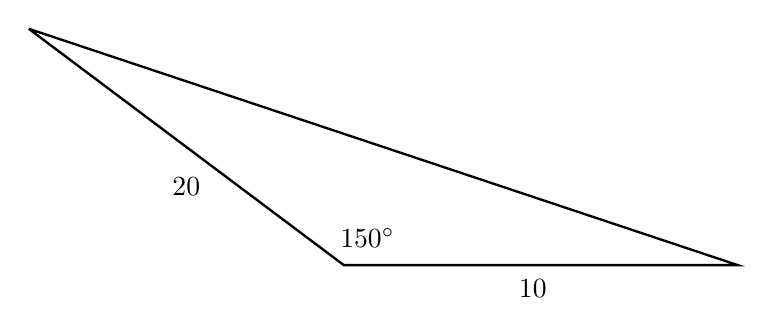
\begin{tikzpicture}
	\draw[line width=0.03cm] (-4,3) -- (0,0) -- (5,0) -- (-4,3);
	\node at (0.3,0.35) {$150^\circ$};
	\node at (2.4,-0.3) {$10$};
	\node at (-2,1) {$20$};
	\end{tikzpicture}
	\] \pspace

{\itshape \sol Dropping a perpendicular from the upper-left most vertex, we can construct the right triangle shown below with angle $\theta$. 
	\[
	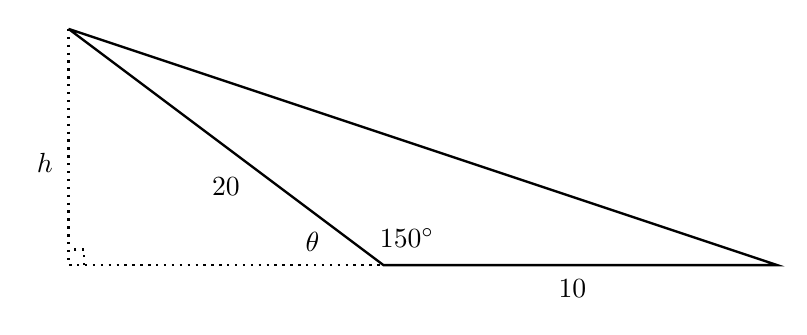
\begin{tikzpicture}
	\draw[line width=0.03cm] (-4,3) -- (0,0) -- (5,0) -- (-4,3);
	\draw[line width=0.03cm,dotted] (-4,3) -- (-4,0) -- (0,0);
	\draw[line width=0.03cm,dotted] (-3.8,0) -- (-3.8,0.2) -- (-4,0.2);
	\node at (-0.9,0.3) {$\theta$};
	\node at (-4.3,1.3) {$h$};
	\node at (0.3,0.35) {$150^\circ$};
	\node at (2.4,-0.3) {$10$};
	\node at (-2,1) {$20$};
	\end{tikzpicture}
	\]
Using the fact that $\theta + 150^\circ= 180^\circ$, we know that $\theta= 30^\circ$. We know that $\sin \theta= \text{opposite}/\text{hypotenuse}$, we have\dots
	\[
	\begin{aligned}
	\sin \theta&= \dfrac{\text{opposite}}{\text{hypotenuse}} \\[0.3cm]
	\sin \left(30^\circ \right)&= \dfrac{h}{20} \\[0.3cm]
	 \dfrac{1}{2}&= \dfrac{h}{20} \\[0.3cm]
	20 \cdot \dfrac{1}{2}&= \dfrac{h}{20} \cdot 20 \\[0.3cm]
	h&= 10
	\end{aligned}
	\]
But then we have\dots
	\[
	A= \dfrac{1}{2}\, bh= \dfrac{1}{2} \cdot 10 \cdot 10= 5 \cdot 10= 50
	\]
Note: One could also use\dots
	\[
	A= \frac{1}{2}\, ab \sin C= \frac{1}{2} \cdot 20 \cdot 10 \sin(150^\circ)= \frac{1}{2} \cdot 20 \cdot 10 \cdot \frac{1}{2}= 10 \cdot 5= 50 
	\]
}



% Question 9
\newpage
\question[10] Compute the exact area of the triangle shown below.
	\[
	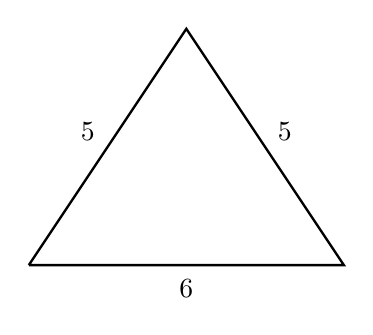
\begin{tikzpicture}
	\draw[line width=0.03cm] (-2,0) -- (0,3) -- (2,0) -- (-2,0);
	\node at (-1.25,1.7) {$5$};
	\node at (1.25,1.7) {$5$};
	\node at (0,-0.3) {$6$};
	\end{tikzpicture}
	\] \pspace

{\itshape \sol To use Heron's area formula, we first find the semiperimeter\dots \pspace
	\[
	s= \dfrac{a + b + c}{2}= \dfrac{5 + 5 + 6}{2}= \dfrac{16}{2}= 8
	\] \pspace
But then by Heron's area formula, we have\dots \pspace
	\[
	A= \sqrt{s(s - a)(s - b)(s - c)}= \sqrt{8(8 - 5)(8 - 5)(8 - 6)}= \sqrt{8 \cdot 3 \cdot 3 \cdot 2}= \sqrt{144}= 12
	\] \pspace
	
	\begin{center} {\bfseries OR} \end{center}

Observe that the triangle is isosceles, dropping a perpendicular from the uppermost vertex bisects the corresponding side. But this gives us the triangle below. 
	\[
	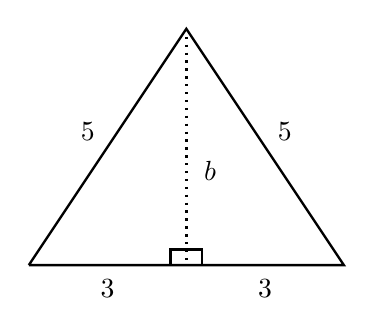
\begin{tikzpicture}
	\draw[line width=0.03cm] (-2,0) -- (0,3) -- (2,0) -- (-2,0);
	\draw[line width=0.03cm] (-0.2,0) -- (-0.2,0.2) -- (0.2,0.2) -- (0.2,0);
	\draw[line width=0.03cm,dotted] (0,3) -- (0,0);
	\node at (-1.25,1.7) {$5$};
	\node at (1.25,1.7) {$5$};
	\node at (-1,-0.3) {$3$};
	\node at (1,-0.3) {$3$};
	\node at (0.3,1.2) {$b$};
	\end{tikzpicture}
	\] 
Using the Pythagorean Theorem, we have $a^2 + b^2= c^2$. But then we have $3^2 + b^2= 5^2$. This implies that $b^2= 16$, so that $b= 4$. But then we have\dots
	\[
	A= \dfrac{1}{2}\, bh= \dfrac{1}{2} \cdot 6 \cdot 4= 3 \cdot 4= 12
	\]
}



% Question 10
\newpage
\question[10] Find the exact value of the side $s$ in the triangle below. 
	\[
	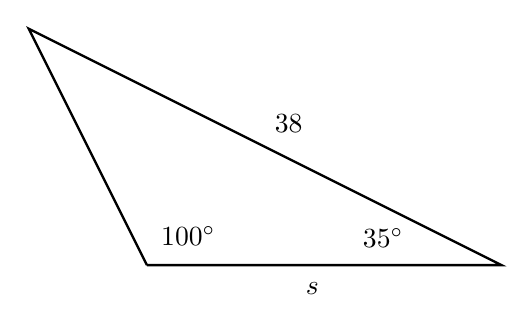
\begin{tikzpicture}[scale=1.5]
	\draw[line width=0.03cm] (-1,0) -- (-2,2) -- (2,0) -- (-1,0);
	\node at (-0.65,0.25) {$100^\circ$};
	\node at (1.0,0.23) {$35^\circ$};
	\node at (0.2,1.2) {$38$};
	\node at (0.4,-0.2) {$s$};
	\end{tikzpicture}
	\] \pspace

{\itshape \sol Because the sum of the angles of a triangle is $180^\circ$, we know the upper-left angle is $180^\circ - 100^\circ - 35^\circ= 45^\circ$. This gives the triangle below:
	\[
	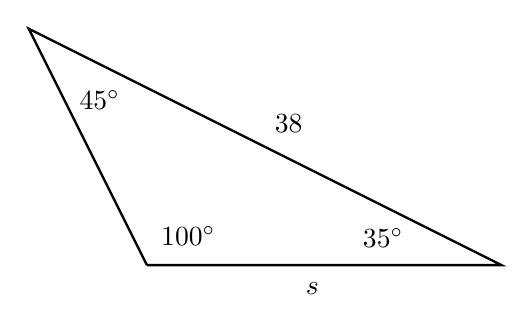
\begin{tikzpicture}[scale=1.5]
	\draw[line width=0.03cm] (-1,0) -- (-2,2) -- (2,0) -- (-1,0);
	\node at (-0.65,0.25) {$100^\circ$};
	\node at (1.0,0.23) {$35^\circ$};
	\node at (0.2,1.2) {$38$};
	\node at (0.4,-0.2) {$s$};
	\node at (-1.4,1.4) {$45^\circ$};
	\end{tikzpicture}
	\] 
Using the Law of Sines, we have\dots
	\[
	\begin{aligned}
	\dfrac{\sin A}{a}&= \dfrac{\sin B}{b} \\[0.3cm]
	\dfrac{\sin(45^\circ)}{s}&= \dfrac{\sin(100^\circ)}{38} \\[0.3cm]
	s \cdot \sin(100^\circ)&= 38 \sin(45^\circ) \\[0.3cm] 
	s&= \dfrac{38 \sin(45^\circ)}{\sin(100^\circ)} \\[0.3cm]
	s&= \dfrac{38 \cdot 1/\sqrt{2})}{\sin(100^\circ)} \\[0.3cm]
	s&= \dfrac{38}{\sqrt{2} \sin(100^\circ)}
	\end{aligned}
	\]
}



% Question 11
\newpage
\question[10] Find the exact value of the side $s$ in the triangle below.
	\[
	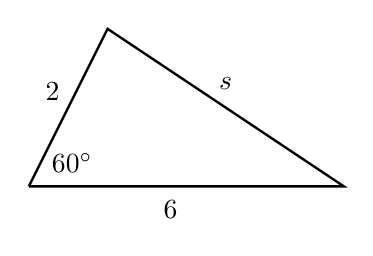
\begin{tikzpicture}
	\draw[line width=0.03cm] (0,0) -- (1,2) -- (4,0) -- (0,0);
	\node at (0.55,0.3) {$60^\circ$};
	\node at (0.3,1.2) {$2$};
	\node at (1.8,-0.3) {$6$};
	\node at (2.5,1.3) {$s$};
	\end{tikzpicture}
	\] \pspace

{\itshape \sol Using the Law of Cosine, we have\dots
	\[
	\begin{aligned}
	c^2&= a^2 + b^2 - 2ab \cos C \\[0.3cm]
	s^2&= 2^2 + 6^2 - 2 \cdot 2 \cdot 6 \cos(60^\circ) \\[0.3cm]
	s^2&= 4 + 36 - 24 \cdot \dfrac{1}{2} \\[0.3cm]
	s^2&= 40 - 12 \\[0.3cm]
	s^2&= 28 \\[0.3cm]
	s&= \sqrt{28} \\[0.3cm]
	s&= 2 \sqrt{7}
	\end{aligned}
	\]
}



% Question 12
\newpage
\question[10] Verify the trigonometric identity given below.
	\[
	\dfrac{\tan \theta - \cot \theta}{\sin \theta \cos \theta}= \sec^2 \theta - \csc^2 \theta
	\] 

{\itshape \sol We have\dots
	\[
	\begin{aligned}
	\dfrac{\tan \theta - \cot \theta}{\sin \theta \cos \theta}&= \dfrac{\tan \theta}{\sin \theta \cos \theta} - \dfrac{\cot \theta}{\sin \theta \cos \theta} \\[0.3cm]
	&= \dfrac{\sin \theta}{\cos \theta} \cdot \dfrac{1}{\sin \theta \cos \theta} - \dfrac{\cos \theta}{\sin \theta} \cdot \dfrac{1}{\sin \theta \cos \theta} \\[0.3cm]
	&= \dfrac{\sin \theta}{\sin \theta} \cdot \dfrac{1}{\cos \theta \cdot \cos \theta} - \dfrac{\cos \theta}{\cos \theta} \cdot \dfrac{1}{\sin \theta \cdot \sin \theta} \\[0.3cm]
	&= \dfrac{1}{\cos^2 \theta} - \dfrac{1}{\sin^2 \theta} \\[0.3cm]
	&= \sec^2 \theta - \csc^2 \theta
	\end{aligned}
	\] 
	\begin{center} {\bfseries OR} \end{center}
We have\dots
	\[
	\begin{aligned}
	\sec^2 \theta - \csc^2\theta&= \dfrac{1}{\cos^2 \theta} - \dfrac{1}{\sin^2 \theta} \\[0.3cm]
	&= \dfrac{1}{\cos^2 \theta} \cdot \dfrac{\sin^2 \theta}{\sin^2 \theta} - \dfrac{1}{\sin^2 \theta} \cdot \dfrac{\cos^2 \theta}{\cos^2 \theta} \\[0.3cm]
	&= \dfrac{\sin^2 \theta}{\sin^2 \theta \cos^2 \theta} - \dfrac{\cos^2 \theta}{\sin^2 \theta \cos^2 \theta} \\[0.3cm]
	&= \dfrac{\sin^2 \theta - \cos^2 \theta}{\sin^2 \theta \cos^2 \theta} \\[0.3cm]
	&= \dfrac{\sin^2 \theta - \cos^2 \theta}{\sin \theta \cos \theta \cdot \sin \theta \cos \theta} \\[0.3cm]
	&= \dfrac{1}{\sin \theta \cos \theta} \cdot \dfrac{\sin^2 \theta - \cos^2 \theta}{\sin \theta \cos \theta} \\[0.3cm]
	&= \dfrac{1}{\sin \theta \cos \theta} \left( \dfrac{\sin^2 \theta}{\sin \theta \cos \theta} - \dfrac{\cos^2 \theta}{\sin \theta \cos \theta} \right) \\[0.3cm]
	&= \dfrac{1}{\sin \theta \cos \theta} \left( \dfrac{\sin \theta}{\cos \theta} - \dfrac{\cos \theta}{\sin \theta} \right) \\[0.3cm]
	&= \dfrac{1}{\sin \theta \cos \theta} \left( \tan \theta - \cot \theta \right) \\[0.3cm]
	&= \dfrac{\tan \theta - \cot \theta}{\sin \theta \cos \theta}
	\end{aligned}
	\]
}



% Question 13
\newpage
\question[10] Verify the trigonometric identity given below.
	\[
	\dfrac{\sin x}{1 + \cos x} + \dfrac{\cos x - 1}{\sin x}= 0 
	\] \pspace

{\itshape \sol We have\dots
	\[
	\begin{aligned}
	\dfrac{\sin x}{1 + \cos x} + \dfrac{\cos x - 1}{\sin x}&= \dfrac{\sin x}{1 + \cos x} \cdot \dfrac{\sin x}{\sin x} + \dfrac{\cos x - 1}{\sin x} \cdot \dfrac{1 + \cos x}{1 + \cos x} \\[0.3cm]
	&= \dfrac{\sin^2 x}{\sin(x) \cdot (1 + \cos x)} + \dfrac{(\cos x - 1)(1 + \cos x)}{\sin(x) \cdot (1 + \cos x)} \\[0.3cm]
	&= \dfrac{\sin^2 x + (\cos x - 1)(1 + \cos x)}{\sin(x) \cdot (1 + \cos x)} \\[0.3cm]
	&= \dfrac{\sin^2 x + (\cos x + \cos^2 x - 1 - \cos x)}{\sin(x) \cdot (1 + \cos x)} \\[0.3cm]
	&= \dfrac{\sin^2 x + (\cos^2 x - 1)}{\sin(x) \cdot (1 + \cos x)} \\[0.3cm]
	&= \dfrac{\sin^2 x - (1 - \cos^2 x)}{\sin(x) \cdot (1 + \cos x)} \\[0.3cm]
	&= \dfrac{\sin^2 x - \sin^2 x}{\sin(x) \cdot (1 + \cos x)} \\[0.3cm]
	&= 0
	\end{aligned}
	\]
}



% Question 14
\newpage
\question[10] Find all the exact solutions to the equation below.
	\[
	3\sin \theta= \sqrt{3} \cos \theta
	\] \pspace

{\itshape \sol Note that $\cos \theta$ and $\sin \theta$ cannot simultaneously vanish. Therefore, both sides cannot be zero at the same time. Then there can be no solutions when $\cos \theta= 0$. We can assume then that $\cos \theta \neq 0$. We have\dots
	\[
	\begin{aligned}
	3\sin \theta&= \sqrt{3} \cos \theta \\[0.3cm]
	\dfrac{3\sin \theta}{\cos \theta}&= \dfrac{\sqrt{3} \cos \theta}{\cos \theta} \\[0.3cm]
	3 \tan \theta&= \sqrt{3} \\[0.3cm] 
	\dfrac{3 \tan \theta}{3}&= \dfrac{\sqrt{3}}{3} \\[0.3cm] 
	\tan \theta&= \dfrac{1}{\sqrt{3}} 
	\end{aligned}
	\]
But the angles $\theta$ with $0 \leq \theta < 2\pi$ such that $\tan \theta= \frac{1}{\sqrt{3}}$ are $\theta= \frac{\pi}{6}$ and $\theta= \frac{7\pi}{6}$. Observe that $\frac{\pi}{6} + \pi= \frac{7\pi}{6}$. The period of $\tan \theta$ is $\pi$. Therefore, the solutions are\dots
	\[
	\theta= \dfrac{\pi}{6} \pm k\pi
	\]
where $k$ is an integer. 
}



% Question 15
\newpage
\question[10] Find all the exact solutions to the equation below.
	\[
	2 \cos(2x) \sin x + \cos(2x)= 0 
	\] \pspace

{\itshape \sol We have\dots
	\[
	\begin{aligned}
	2 \cos(2x) \sin x + \cos(2x)&= 0 \\[0.3cm]
	\cos(2x) \cdot (2 \sin x + 1)&= 0 
	\end{aligned}
	\] \pspace
But then either $\cos(2x)= 0$ or $2 \sin x + 1= 0$. If $\cos(2x)= 0$ and $0 \leq 2x < 2\pi$, we know $2x= \frac{\pi}{2}$, so that $x= \frac{\pi}{4}$, or $2x= \frac{3\pi}{2}$, so that $x= \frac{3\pi}{4}$. The period of $\cos(x)$ is $2\pi$ so that the period of $\cos(2x)$ is $\pi$. But then the solutions to $\cos(2x)= 0$ are $x= \frac{\pi}{4} \pm k\pi$ and $x= \frac{3\pi}{4} \pm k\pi$, where $k$ is an integer. \pspace

If $2\sin x + 1= 0$, then we know that $2\sin x= -1$ so that $\sin x= -\frac{1}{2}$. If $\sin x= -\frac{1}{2}$ and $0 \leq x < 2\pi$, then $x= \frac{7\pi}{6}$ or $x= \frac{11\pi}{6}$. Because the period of $\sin x$ is $2\pi$, the solutions to $\sin x= -\frac{1}{2}$ are $x= \frac{7\pi}{6} \pm 2\pi k$ and $x= \frac{11\pi}{6} \pm 2\pi k$, where $k$ is an integer. \pspace

Therefore, the solutions are\dots
	\[
	\begin{aligned}
	x&= \frac{\pi}{4} \pm k\pi \\[0.3cm]
	x&= \frac{3\pi}{4} \pm k\pi \\[0.3cm]
	x&= \frac{7\pi}{6} \pm 2\pi k \\[0.3cm]
	x&= \frac{11\pi}{6} \pm 2\pi k
	\end{aligned} 
	\]
}





























\end{questions}
\end{document}